\subsection{Appendix A - Closure Properties}
\begin{center}
\setlength{\extrarowheight}{.5ex}
\renewcommand{\check}{{\color[HTML]{25c925}\ding{51}}}
\renewcommand{\cross}{{\color{red}\ding{55}}}
\begin{tabular}{|c||c|c|c|c|c|c|}
\hline
             % & union     & intersection & concatenation & star      & complement   & homomorphism \\ \hline \hline
             & $A\cup B$ & $A\cap B$    & $A\cdot B$    & $A^*$     & $\overline{A}$ & homomorphism \\ \hline \hline
Regular      & \check    & \check       & \check        & \check    & \check         & \check       \\ \hline
Context-free & \check    & \cross       & \check        & \check    & \cross         & \check       \\ \hline
Decidable    & \check    & \check       & \check        & \check    & \check         & \cross       \\ \hline
Recognizable & \check    & \check       & \check        & \check    & \cross         & \check       \\ \hline
P            & \check    & \check       & \check        & \check    & \check         & iff P=NP     \\ \hline
NP           & \check    & \check       & \check        & \check    & iff NP=coNP    &              \\ \hline
PSPACE       & \check    & \check       & \check        & \check    & \check         &              \\ \hline
L            & \check    & \check       & \check        & iff L=NL  &                &              \\ \hline
NL           & \check    & \check       & \check        & \check    & \check         &              \\ \hline
BPP          & \check    & \check       &               &           & \check         &              \\ \hline
\end{tabular}
\end{center}

% \begin{center}
% \renewcommand{\check}{{\color[HTML]{25c925}\ding{51}}}
% \renewcommand{\cross}{{\color{red}\ding{55}}}
% \begin{tabular}{|c||c|c|c|c|c|c|}
% \hline
%                      & decidable     & recognizable & co-recognizable  \\ \hline \hline
% \genlang{A}{DFA}     & \check        & \check       & \check           \\ \hline
% \genlang{E}{DFA}     & \check        & \check       & \check           \\ \hline
% \genlang{ALL}{DFA}   & \check        & \check       & \check           \\ \hline
% \genlang{EQ}{DFA}    & \check        & \check       & \check           \\ \hline
% \genlang{HALT}{DFA}  & \check        & \check       & \check           \\ \hline \hline
                                                                                
% \genlang{A}{CFG}     & \check        & \check       & \check           \\ \hline
% \genlang{E}{CFG}     & \check        & \check       & \check           \\ \hline
% \genlang{ALL}{CFG}   & \check        & \check       & \check           \\ \hline
% \genlang{EQ}{CFG}    & \check        & \check       & \check           \\ \hline
% \genlang{HALT}{CFG}  & \check        & \check       & \check           \\ \hline \hline
                                                                                
% \genlang{A}{LBA}     & \check        & \check       & \check           \\ \hline
% \genlang{E}{LBA}     & \check        & \check       & \check           \\ \hline
% \genlang{ALL}{LBA}   & \check        & \check       & \check           \\ \hline
% \genlang{EQ}{LBA}    & \check        & \check       & \check           \\ \hline
% \genlang{HALT}{LBA}  & \check        & \check       & \check           \\ \hline \hline
                                                                                
% \genlang{A}{TM}      & \check        & \check       & \check           \\ \hline
% \genlang{E}{TM}      & \check        & \check       & \check           \\ \hline
% \genlang{ALL}{TM}    & \check        & \check       & \check           \\ \hline
% \genlang{EQ}{TM}     & \check        & \check       & \check           \\ \hline
% \genlang{HALT}{TM}   & \check        & \check       & \check           \\ \hline
% \end{tabular}
% \end{center}

% \vspace{1em}

\subsection{Appendix B - Classes Hierarchies}
\begin{center}
\begin{large}
Regular $\subset$ Context-free $\subset$ Decidable $\subset$ Turing-recognizable
\newcommand{\verteq}{\rotatebox{90}{$\,=$}}
\newcommand{\equalto}[2]{\underset{\scriptstyle\overset{\mkern4mu\verteq}{#2}}{#1}}
\[
    \classl \subseteq \equalto{\classnl}{\text{coNL}} \subseteq \classp \subseteq \classnp \subseteq \equalto{\text{PSPACE}}{\text{NPSPACE}} \subseteq \text{EXPTIME} \subseteq \equalto{\text{EXPSPACE}}{\text{NEXPSPACE}}
\]
\vspace{2em}
\begin{footnotesize}
    Note: NL $\subsetneq$ PSPACE,$\quad$ P $\subsetneq$ EXPTIME,$\quad$ PSPACE $\subsetneq$ EXPSPACE
\end{footnotesize}
\end{large}

\vspace{1em}

\begin{figure}[!ht]
    \centering
    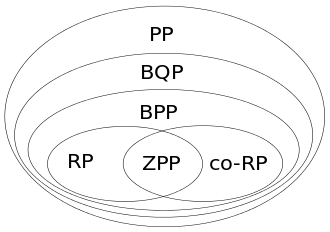
\includegraphics[width=0.45\textwidth]{Computation/claims/hierarchies/bpp.png}
    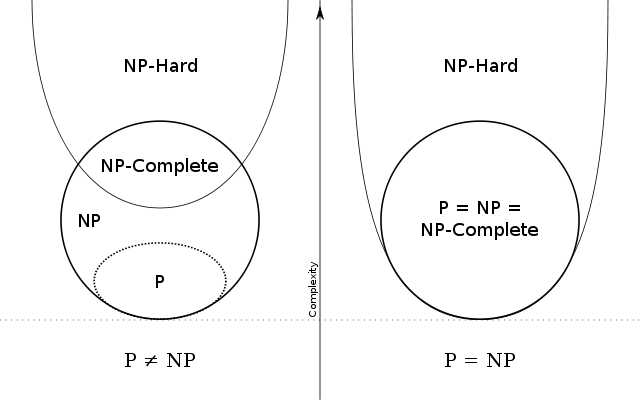
\includegraphics[width=0.5\textwidth]{Computation/claims/hierarchies/fig2.png}
    % \caption{Class hierarchies}
\end{figure}

\clearpage

\begin{figure}[!ht]
    \centering
    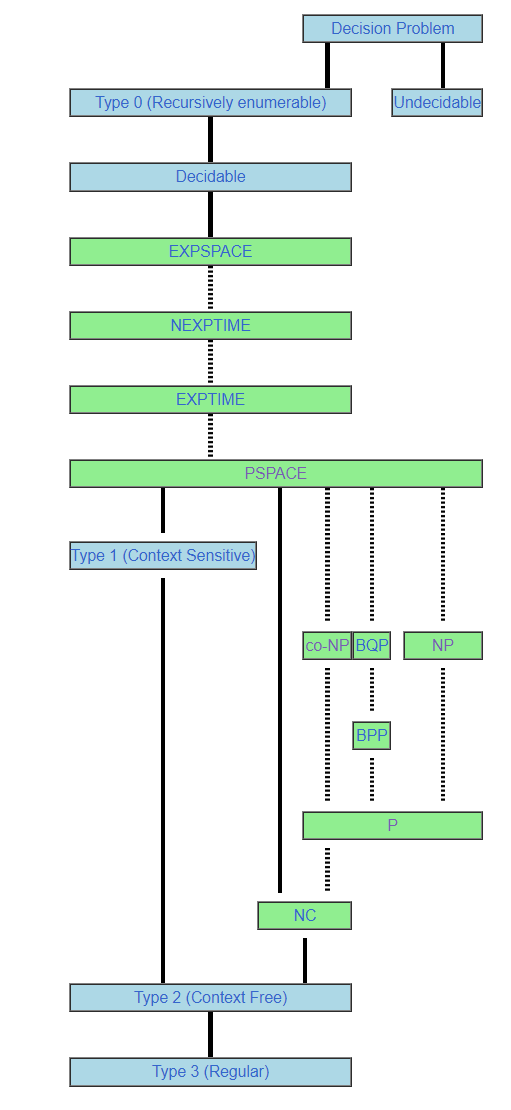
\includegraphics[width=0.45\textheight]{Computation/claims/hierarchies/fig3.png}
    % \caption{More class hierarchies}
\end{figure}

\end{center}

% \subsection{Appendix C - Mamans}